% Section 5 - The tf2 library
% Roberto Masocco <roberto.masocco@uniroma2.it>
% June 5, 2024

% ### The tf2 library ###
\section{The tf2 library}
\graphicspath{{figs/section5/}}

% --- Rigid transformations ---
\begin{frame}{Rigid transformations}
	When a robot moves in space, it is important to keep track of its \textbg{position} and \textbg{orientation} with respect to a \textbg{reference frame}.\\
	\bigskip
	Sensors measuring this information, as well as many more, are \textbg{mounted} on the robot, in fixed positions and orientations.\\
	\bigskip
	To process these measurements, they must first be \textbg{transformed} from the \textbg{body frame} into a common reference frame, usually called:
	\begin{itemize}
		\item \textbg{world frame} (world origin), in the case of \textbg{global localization};
		\item \textbg{local frame}, or \textbg{odom frame} (robot starting point), in the case of \textbg{local localization}.
	\end{itemize}
	\medskip
	Such \textbg{rigid transformations} are \textbg{isometries}. They must be applied to almost every sensor measurement, and are usually \textbg{composable}.\\
	\bigskip
	We would like the middleware to provide tools to do this almost automatically...
\end{frame}

% --- The tf2 library ---
\begin{frame}{The tf2 library}
	\begin{columns}
		\column{.6\textwidth}
		\texttt{tf2} is the \textbg{standard ROS 2 library} to handle rigid transformations.\\
		\medskip
		It allows to:
		\begin{itemize}
			\item \textbg{broadcast} and \textbg{listen} to transformations, thanks to appropriate buffering subscribers and publishers;
			\item \textbg{transform} any kind of sensor data from one frame to another, making efficient computations in C++ code relying on the \texttt{Eigen} mathematical library;
			\item broadcast \textbg{robot descriptions} from \texttt{URDF} files, listing links and joints and how they are connected, resulting in a \textbg{tree-like structure};
			\item \textbg{command-line tools} to inspect the current tree status, and broadcast custom transformations.
		\end{itemize}

		\column{.4\textwidth}
		\begin{figure}
			\centering
			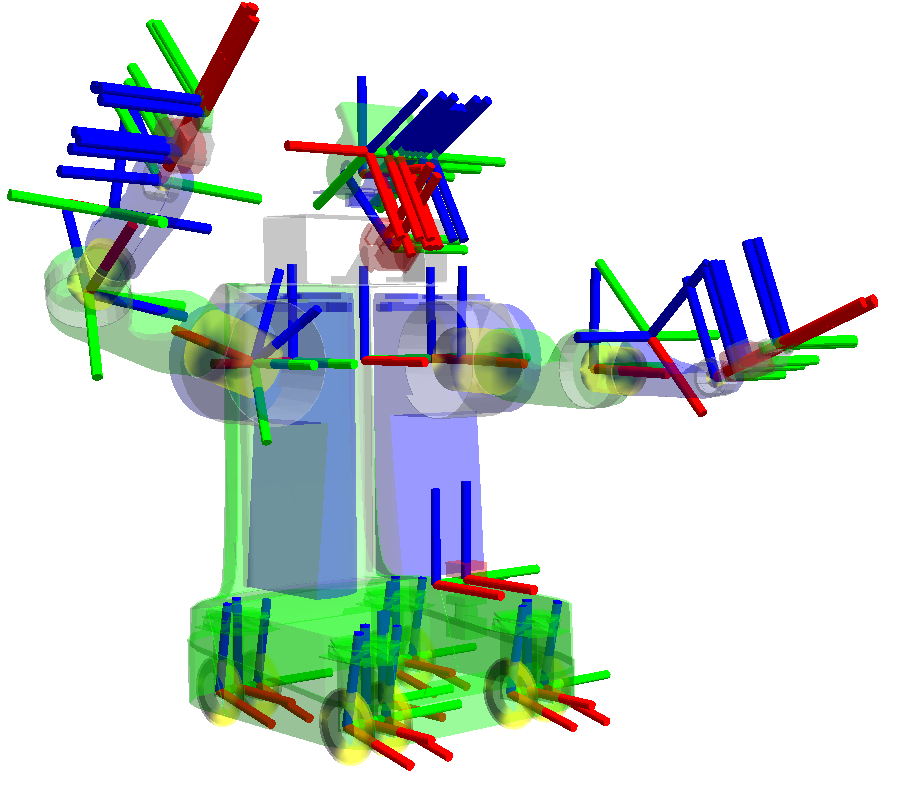
\includegraphics[width=.9\textwidth]{ros2_tf2}
			\caption{Example of robot description with tf2.}
			\label{fig:tf2example}
		\end{figure}
	\end{columns}
\end{frame}
\begin{frame}{The tf2 library}
	\begin{figure}
		\centering
		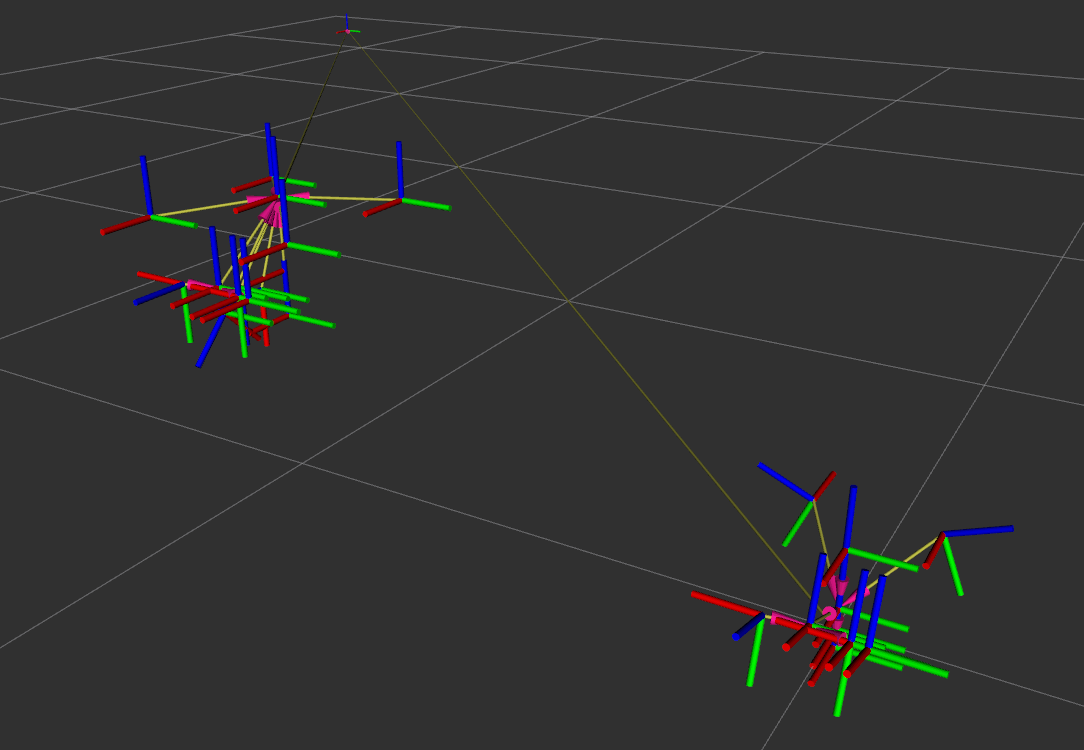
\includegraphics[width=.58\textwidth]{tfs}
		\caption{Broadcasted robot descriptions, plus real-time transformations given by localization systems.}
		\label{fig:tfs}
	\end{figure}
\end{frame}
